\chapter{Extensions of OverCode Clustering}\label{chapter:grovercode}

The original vision of OverCode was to discover pedagogically valuable themes of variation within thousands of student solutions to the same programming exercise. While OverCode does canonicalize and cluster correct solutions so that they can be more easily understood as a group, it does not pull out larger themes of variation as clearly as initially hoped for, nor does it handle incorrect solutions. This chapter describes more recent efforts to address both these shortcomings.

\section{Clustering Solutions with Statistical Models}\label{sec:latent}

One approach to pulling out larger themes of variation within solutions is to cluster more aggressively. OverCode's existing clustering pipeline is a form of deterministic interpretable clustering. What can vary and what is invariant across all the solutions within a cluster is clear, just by reading the canonicalized solution that represents the cluster. Because it faithfully represents the syntax students used in each cluster, solutions are split apart into smaller clusters by small syntactic differences. 

One promising set of methods for more aggressive groupings of solutions are bottom-up and rule-based: they define rules for which solutions or groups of solutions can be merged into a single cluster. Probablistic semantic equality or equality with respect to a teacher's test suite, which is already used by OverCode for variable names, can be used for subexpressions as well~\cite{}. Programming language-based methods, e.g., compiler optimizations, could collapse OverCode clusters based on known semantic equality. As a system designer, one must decide or give the teacher control over how many different, semantically equivalent solutions are collapsed into a single cluster since, at the highest level, all correct solutions to the same programming exercise are semantically equivalent. These methods are discussed again in the future work, because the second set of methods were chosen for future investigation in this chapter.

The second set of methods leverage statistical properties of the entire corpus of solutions. Given that Variation Theory is interested in dimensions of variation (and consistency) that characterize all possible instantiations of an idea, statistical methods warrant further investigation. Latent variable models are a type of statistical model that attempt to explain variation in a dataset based on underlying factors. With the right choice of features and model, a latent variable model may be able to capture underlying design choices. In this section, two latent variable models have been explored in a preliminary way for this purpose: the Bayesian Case Model (BCM)~\cite{} and Latent Dirichlet Allocation (LDA)~\cite. 

BCM was selected because, like the original OverCode pipeline, it clusters solutions and produces a single solution to represent the entire cluster. Like OverCode, it also indicates the features that characterize each cluster. While OverCode displays the set of canonicalized lines that all members of a cluster deterministically share, BCM learns a subspace of features that are most characteristic of the solutions within cluster, in a probabilistic sense. It also has an interactive variant called iBCM, which allows the user to directly modify the prototype and the subspace chosen by BCM if it disagrees with their domain knowledge or preferences. This user modification triggers a rerun of BCM with the modifications taken into account.%is taken into account by the algorithm 

Internally, BCM depends on a mixture model with a Dirichlet prior. Rather than find a cluster for each entire solution, mixture models can learn clusters of features that co-exist across some subset of all solutions. The concentration parameter of BCM's Dirichlet prior is set to promote sparsity, i.e., mixture distributions over solutions that have the majority of their probability mass on a single mixture component. BCM then assigns each solution to a cluster according to its most probable mixture component. %In other words, after fitting the model to the data, each solution will likely have a single dominant mixture component associated with it. If data points were documents instead of solutions, one would say that each document is determined to have a single dominating topic.

LDA was selected as an alternative statistical approach to BCM because of evidence collected at UCBerkeley~\cite{} that experts were themselves not particularly consistent about how to cluster solutions. While LDA's output is not as optimized for interpretability as BCM's, it preserves the ability to examine solutions through the lens of their mixture components, rather than clusters. LDA learns both mixture components, which are distribution over features, and the distributions of those mixtures over each solution in the set it is trained on. Depending on the features chosen to represent solutions, it may be difficult to interpret exactly what a mixture component is just by looking at its distribution over features. However, sorting solutions based on the degree to which a particular topic is associated with them may pull out a distinctive, human-interpretable themes. %Furthermore, when using LDA, the concentration parameter of the Dirichlet prior need not promote for sparsity; it can be tuned by a human or a heuristic, to maximize the usefulness of the resulting breakdown into mixture components. This parameter's optimal value may be problem-specific and teacher-specific. 



\subsection{Interpretable Clustering Solutions with BCM}

BCM was applied to the canonicalized cluster-representing solutions generated by OverCode. These canonicalized solutions encode both static and dynamic information in a readable function, i.e., the syntax carries the static information and the variable name encodes dynamic information. The canonicalized function body is tokenized and represented as binary vectors indicating  the existence of the features, including renamed variables and language-specific keywords, such as specific canonicalized variable names like \texttt{listA} and Python keywords like \texttt{assert} and \texttt{while}. The result is a BCM clustering of OverCode clusters.

In a small pilot study, three introductory Python teachers were each given sets of Python solutions to three different programming problems selected from those previously analyzed in the chapter on OverCode. For each problem, they were asked to create a grading rubric and provide helpful comments for the students, based on interacting with solutions in one of three different interfaces. The three interfaces were: (1) raw solutions in the browser, similar to the control used in the OverCode studies, (2) OverCode's canonicalized cluster-representating solutions, and (3) a BCM clustering of OverCode clusters, i.e., the prototypes and characteristic features of each BCM cluster, as well as its cluster members. The BCM interface, shown in Figure~\ref{overcode_ibcm}, was running the iBCM variant of the algorithm, so teachers could promote a member of a cluster to be its prototype or click on a token within a prototype--a variable name or keyword--to toggle whether or not it is considered a characteristic feature of that cluster. Both these modifications triggered BCM running in the backend to rerun and send a new clustering to the front end for display. 

Pilot users appreciated the fact that BCM gave some structure to the space of solutions; rather than a long list of solutions, the interface suggested distinct subpopulations of solutions within the list. However, subjects did not fully understand the probabilistic nature of the clustering method. The presence of a single "intruder", i.e., a solution that the teacher believed did not belong in a cluster, caused confusion. This could be ameliorated by giving users more ways to modify the clustering, e.g., allowing users the option to kick an intruder out of a cluster and rerun BCM, or by introducing the tool as a mechanism for "discovery" instead of "organization." Subjects also requested richer or higher-level features than variable names and keywords. Kim's PhD thesis~\cite{beenthesis} describes a follow-up full user study comparing the efficacy of BCM vs. iBCM on clustering OverCode cluster-representing solutions.

\begin{figure}[ht]
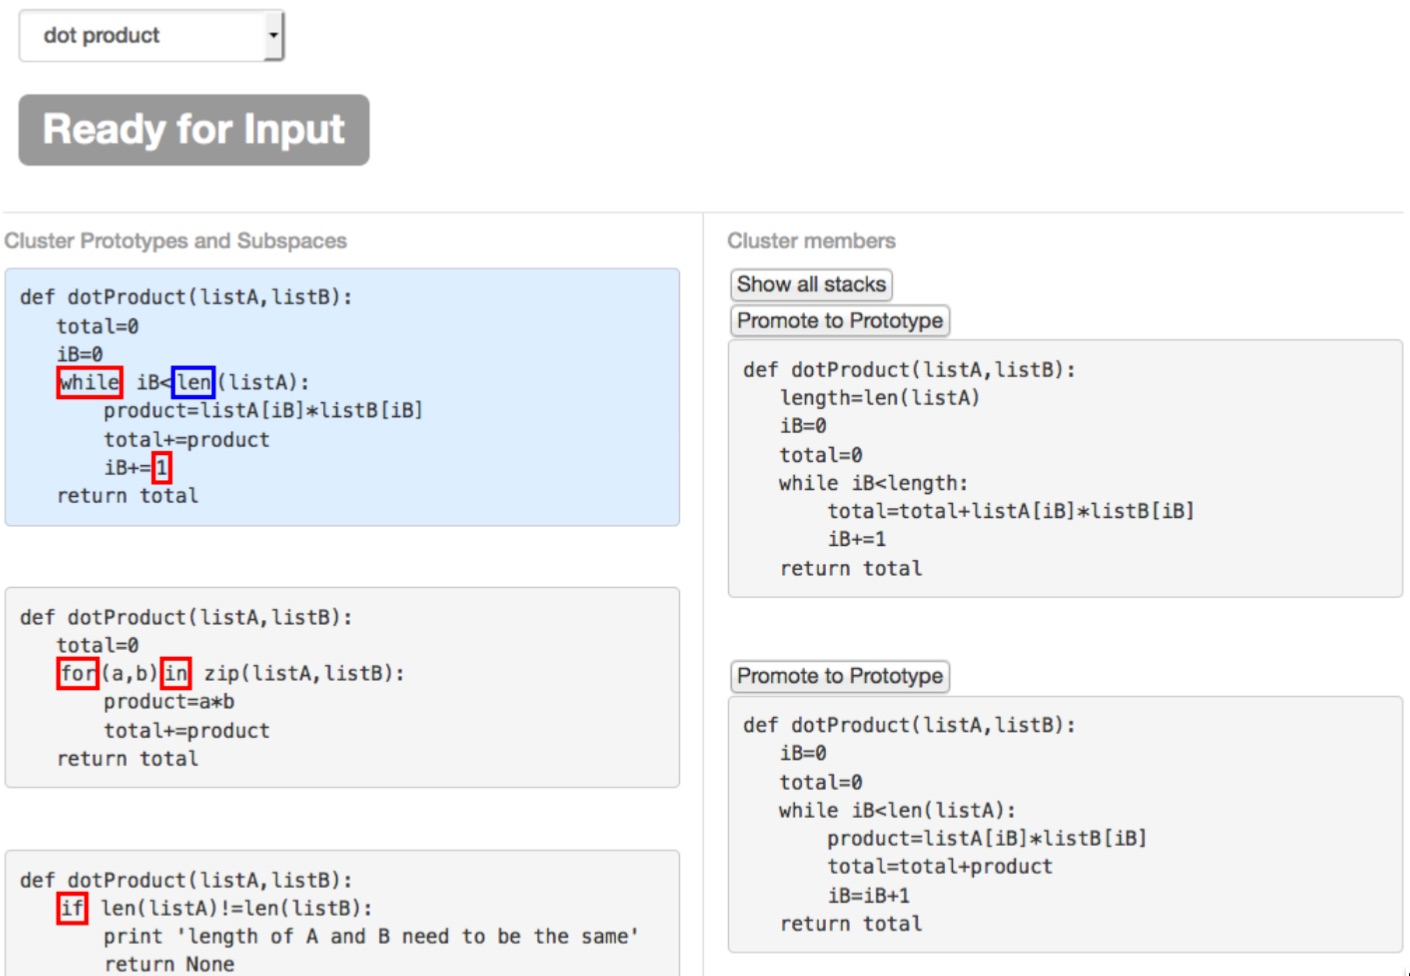
\includegraphics[width=0.75\columnwidth]{Body/figures/grovercode/overcode_ibcm}
\caption{The solutions on the left are cluster prototypes. The blue solution is the selected cluster whose members are shown in a scrollable list on the right hand side. The tokens contained in red boxes are features that BCM "believes" characterize the cluster represented by that prototype. When a user hovers their cursor over a keyword or variable name, e.g., \texttt{len}, it is highlighted in a blue rectangle, indicating that it can be interacted with, i.e., clicked.}
\label{overcode_ibcm}
\end{figure} 

\subsection{Mixture Modeling Solutions with LDA}

As described in the chapter on related work, other researchers have documented a lack of agreement across human-made clusters of student code. One possible explanation for this low consistency across teacher-made clusterings of student code is that solutions are mixtures of design choices and teachers care about different things. As described in~\cite{berkeleymastersthesis}: the clusters can be as straight forward as "1 pt", "2 pts" and "3 pts". If student A writes a solution with a well-written loop and extraneous statements while student B writes a solution with extra loops but otherwise very clean code, teachers can reasonably disagree about which cluster each whole solution should be placed in, depending on whether they believe inefficient control flow or extraneous statements are worse.

Instead of trying to approximate clusterings that humans do not even agree on, it may be more useful to model solutions as mixtures of good and bad design choices. While more sophisticated mixture models' assumptions may ultimately be more appropriate, LDA \cite{lda} as implemented in the Gensim toolbox \cite{gensim} was chosen as the model to evaluate in this preliminary work. 

Like BCM, LDA was run on the canonicalized cluster-representing solutions, not raw solutions. However, the representation of these solutions was also changed: in order to pull out higher-level patterns in approach, rather than lower-level patterns in syntax, solutions were represented solely by the behavior of the variables within them. 

As described in the chapter on OverCode, the OverCode analysis pipeline executes all programs on a common set of test cases and records the sequence of values taken on by each variable in the program. OverCode assumes that variables in different programs that transition through the same sequence of values on the same test cases are in fact fulfilling the same semantic role in the program. %This sequence of values taken on by each variable in each program becomes a signature, i.e., the key to recognizing semantically equivalent variables across programs.  % and can therefore be considered the same {\bf common variable} uniquely defined by that sequence of values.



\begin{figure}[ht]
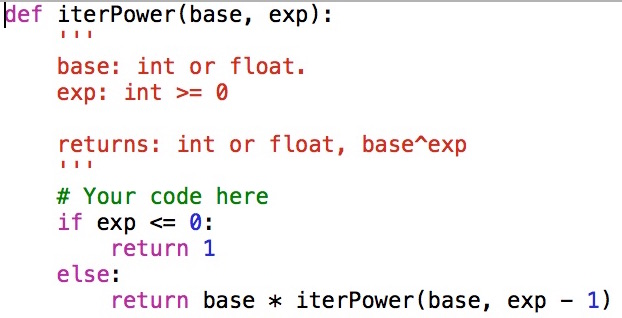
\includegraphics[width=0.75\columnwidth]{Body/figures/grovercode/recursive_example}
\caption{Example of a recursive student solution.}
\label{recursive_example}
\vspace*{\floatsep}
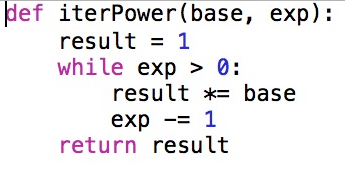
\includegraphics[width=0.45\columnwidth]{Body/figures/grovercode/whilestandard}
\caption{Example of a \texttt{while}-based student solution.}
\label{whilestandard}
\vspace*{\floatsep}
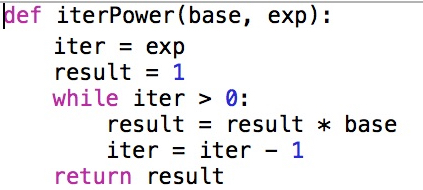
\includegraphics[width=0.5\columnwidth]{Body/figures/grovercode/augmentedwhile}
\caption{Example of a \texttt{while}-based student solution, where the student has not modified any input arguments, i.e., better programming style.}
\label{augmentedwhile}
\end{figure} 

Below are the sequences of variable values recorded by OverCode while executing \texttt{iterPower(5,3)} as defined in Figures \ref{recursive_example}, \ref{whilestandard}, and \ref{augmentedwhile}:
\begin{itemize}
  \item {\bf Figure \ref{recursive_example}}
  \begin{itemize}
  \setlength\itemsep{0.05em}
  \item \texttt{exp: 3, 2, 1, 0, 1, 2, 3}
  \item \texttt{base: 5}
  \end{itemize}
  \item {\bf Figure \ref{whilestandard}}
  \begin{itemize}
  \item \texttt{exp: 3, 2, 1, 0}
  \item \texttt{base: 5}
  \item \texttt{result: 1, 5, 25, 125}
  \end{itemize}
  \item {\bf Figure \ref{augmentedwhile}}
  \begin{itemize}
  \item \texttt{exp: 3}
  \item \texttt{base: 5}
  \item \texttt{iter: 3, 2, 1, 0}
  \item \texttt{result: 1, 5, 25, 125}
  \end{itemize}
\end{itemize}

In the previous examples, the input argument \texttt{base} would be considered variable common to all three programs, but the input argument \texttt{exp} would not be. The variable \texttt{result} would also be considered a common variable shared across just the definitions in Figure \ref{whilestandard} and Figure \ref{augmentedwhile}. This allows us to distinguish between programs that calculate the answer in semantically distinct ways, without discriminating between the low-level syntax-based design decisions. 

LDA is often applied to corpuses of textual documents, where the corpus is represented as a $W \times N$ term-by-document matrix of counts, where $W$ is the vocabulary size across all documents and $N$ is the number of documents. In this representation, the document is represented a bag of word counts, i.e., how many times each word appears in the document. Following this analogy, solutions are represented as a bag of variable behaviors. The matrix representing the solutions in Figures \ref{recursive_example} through \ref{augmentedwhile} executed on \texttt{iterPower(5,3)} is shown in Table \ref{varbydocmat}.

\begin{table}[t]
\caption{Variable-by-Solution Matrix for Programs, where variables are uniquely identified by their sequence of values while run on a set of test case(s)}
\label{varbydocmat}
%\vskip 0.15in
\begin{center}
\begin{small}
\begin{sc}
\begin{tabular}{| l | c | c | c | c | c |}
\hline
%\abovespace\belowspace
Sol- & \texttt{5} & \texttt{1,5,...} & \texttt{3,2,1,0,} & \texttt{3,2,1,0} & \texttt{3} \\
ution& & \texttt{25,125} & \texttt{...1,2,3} & &  \\
\hline
%\abovespace
Fig. \ref{recursive_example} & 1 & 0 & 1 & 0 & 0 \\
Fig. \ref{whilestandard}     & 1 & 1 & 0 & 1 & 0 \\
Fig. \ref{augmentedwhile}    & 1 & 1 & 0 & 1 & 1 \\
\hline
\end{tabular}
\end{sc}
\end{small}
\end{center}
%\vskip -0.1in
\end{table}

Note that, while the entries in Table \ref{varbydocmat} only take on values $0$ or $1$, more complicated definitions may have $n$ instances of, e.g., a variable that takes on the sequence of values \texttt{3,2,1,0}. In that case, there could be an $n$ in the \texttt{3,2,1,0} column for the row corresponding to that solution, or it can be left as a binary indicator. %In other words, true to the assumptions made by LDA, these are occurrence counts, not binary indicators.

%\subsection{Procedure}

In order to run LDA, 3875 student solutions to \texttt{iterPower} were first run on a set of test cases within the OverCode analysis pipeline. The OverCode pipeline produced a set of 977 cluster-representing solutions and a set of features for each solution, including which variable sequences were observed during execution. Another script turned this output into a variable-by-solution matrix for the 977 cluster-representing solutions, which were then fed into LDA for analysis. LDA was run repeatedly with multiple values for the parameter that sets the number of latent mixture components. The results were examined by hand since perplexity and held-out likelihoods are not necessarily good proxies for human interpretability \cite{readingtealeaves}. 

Since the learned mixture components are distributions over variable behaviors, it is easier to inspect solutions which have high "amounts" of that mixture component "within" them and infer a theme by comparing them to solutions that contain high "amounts" of a different mixture component. These comparisons were done by hand for a subset of popular mixture components for each LDA model. One topic comparison captured the difference between solutions like Figure ~\ref{augmentedwhile} and ~\ref{whilestandard}. Another topic comparison exposed the difference between the subpopulation of solutions with extra (unnecessary) conditional statements and the common, more concise solution. In the future, a user interface would be very helpful for this task, especially one which made it easier to compare the output of models with different parameter values. 

LDA applied to a variable-by-solution matrix is a promising method for identifying variation within corpuses of solutions to the same programming exercise. However, LDA's assumptions, such as the independence of mixture components, and requirements, such as explicitly setting the number of mixture components beforehand, may mean that other mixture models, such as the Correlated Topic Model~\cite{} or the Hierarchical Dirichlet Process~\cite{} will ultimately be a better model fit for this purpose.

\section{GroverCode: Clustering and Canonicalizing Incorrect Solutions}\label{sec:grover}

While understanding the contents of thousands of correct student solutions can be helpful in both residential and online contexts, another application of OverCode's pipeline and interface is supporting the hand-grading of introductory Python programming exam solutions, only some of which are correct. Incorrect solutions are defined as those that do not pass at least one test case in the teacher-designed test suite.

Hand-reviewing solutions is necessary because teacher-designed test suites were found to unfairly penalize some students and award undeserved credit to others. For example, a single typo in an otherwise well-written solution can cause it to fail all the test cases and receive no credit. Conversely, a solution that subverts the purpose of the assignment can still receive credit by returning the expected answer to some or all of the test cases.

For the staff of 6.0001, the residential introductory Python programming courses at MIT, this can be one of the most time-consuming and exhausting parts of teaching the course. It can take an full workday for the entire staff of eight to ten teachers to sit in a room and review several hundred students' solutions by hand in order to assign a single numerical grade to each solution. 

There are two main technical contributions found in the GroverCode extension of OverCode: a modified pipeline that can canonicalize both correct and incorrect solutions and an interface designed for grading. Just as the original pipeline used variable behavior to canonicalize variable names, the modified pipeline uses variable behavior and the syntax of statements containing each variable to canonicalize variable names in solutions that are not correct. This comes from the insight that a variable in an incorrect solution can be semantically equivalent to a variable in a correct solution but still behave differently; it can behave differently due to a bug in a line of code that directly modifies its value or a bug in a line of code that affects the behavior of another variable that it depends on. Since many of the exam solutions are incorrect and do not get clustered together, the new user interface organizes solutions according to their behavior on test cases and compositional similarity to each other, rather than by cluster size.

GroverCode was iteratively designed and evaluated as a grading tool through two live deployments during the Spring 2016 6.0001 staff exam grading sessions. Approximately two hundred students were enrolled in the course, and nine instructors used GroverCode to grade nearly all student code submissions. A total of seven programming exercises of a variety of difficulties were graded over the course of these two sessions. GroverCode was particularly appreciated on simpler problems where correct solutions were clustered together and graded by a single teacher's action. The canonicalization process applied to more complex solutions, especially those which included student-written objects, was at times more harmful than helpful for teacher's comprehension of student code. Conversely, the feature for grouping solutions based on their behavior on test cases was appreciated regardless of solution complexity.

\subsection{User Interface}

Figures~\ref{fig:whole_interface},~\ref{fig:correct_stack}, and~\ref{fig:rubric} capture the GroverCode user interface during the second and final deployment of the Spring 2016 term. Unlike OverCode, there are both correct and incorrect solutions in view; they are differentiable by their different background colors, as well as a red "X" next to every failed test. To better explain each test failure, the solution's differing actual and expected outputs are also displayed. 

The panel of progress indicators and filters is always in view. The rows of aligned sequences of green checks and red dashes represent "error vectors", the pass/fail results with respect to the ordered list of teacher-specified test cases. The checkbox next to each error vector allows the teacher to selectively view subsets of solutions based on the particular tests they pass and fail. Solutions with the same error vectors may include similar mistakes.

Correct solutions are stacked the same way they are in OverCode. In contrast, incorrect solutions were canonicalized but not stacked, even if they were identical after canonicalization. Grades are propagated to all the solutions in a stack; propagating actual student grades based on a probabilistic canonicalization process that was not thoroughly vetted before deployment would be unfair to students. 

The user interface includes the following features in an attempt to minimize the cognitive load experienced by teachers rapidly switching between grading one solution and the next:
\begin{itemize}
\item Horizontally aligned solutions for side-by-side comparison
\item Easy filtering of solutions by input-output behavior, i.e., their error vectors
\item Canonicalized variable names
\item Solutions ordered to minimize the distance between adjacent solutions with respect to a custom similarity metric defined in Terman~\ref{staceythesis}
\item Highlighted lines of code in each solution which differ from the previous solution in the horizontal list
\end{itemize}

The hope is that canonicalization helps teachers switch between solutions more often than it harms reability.

\begin{figure}
\centering
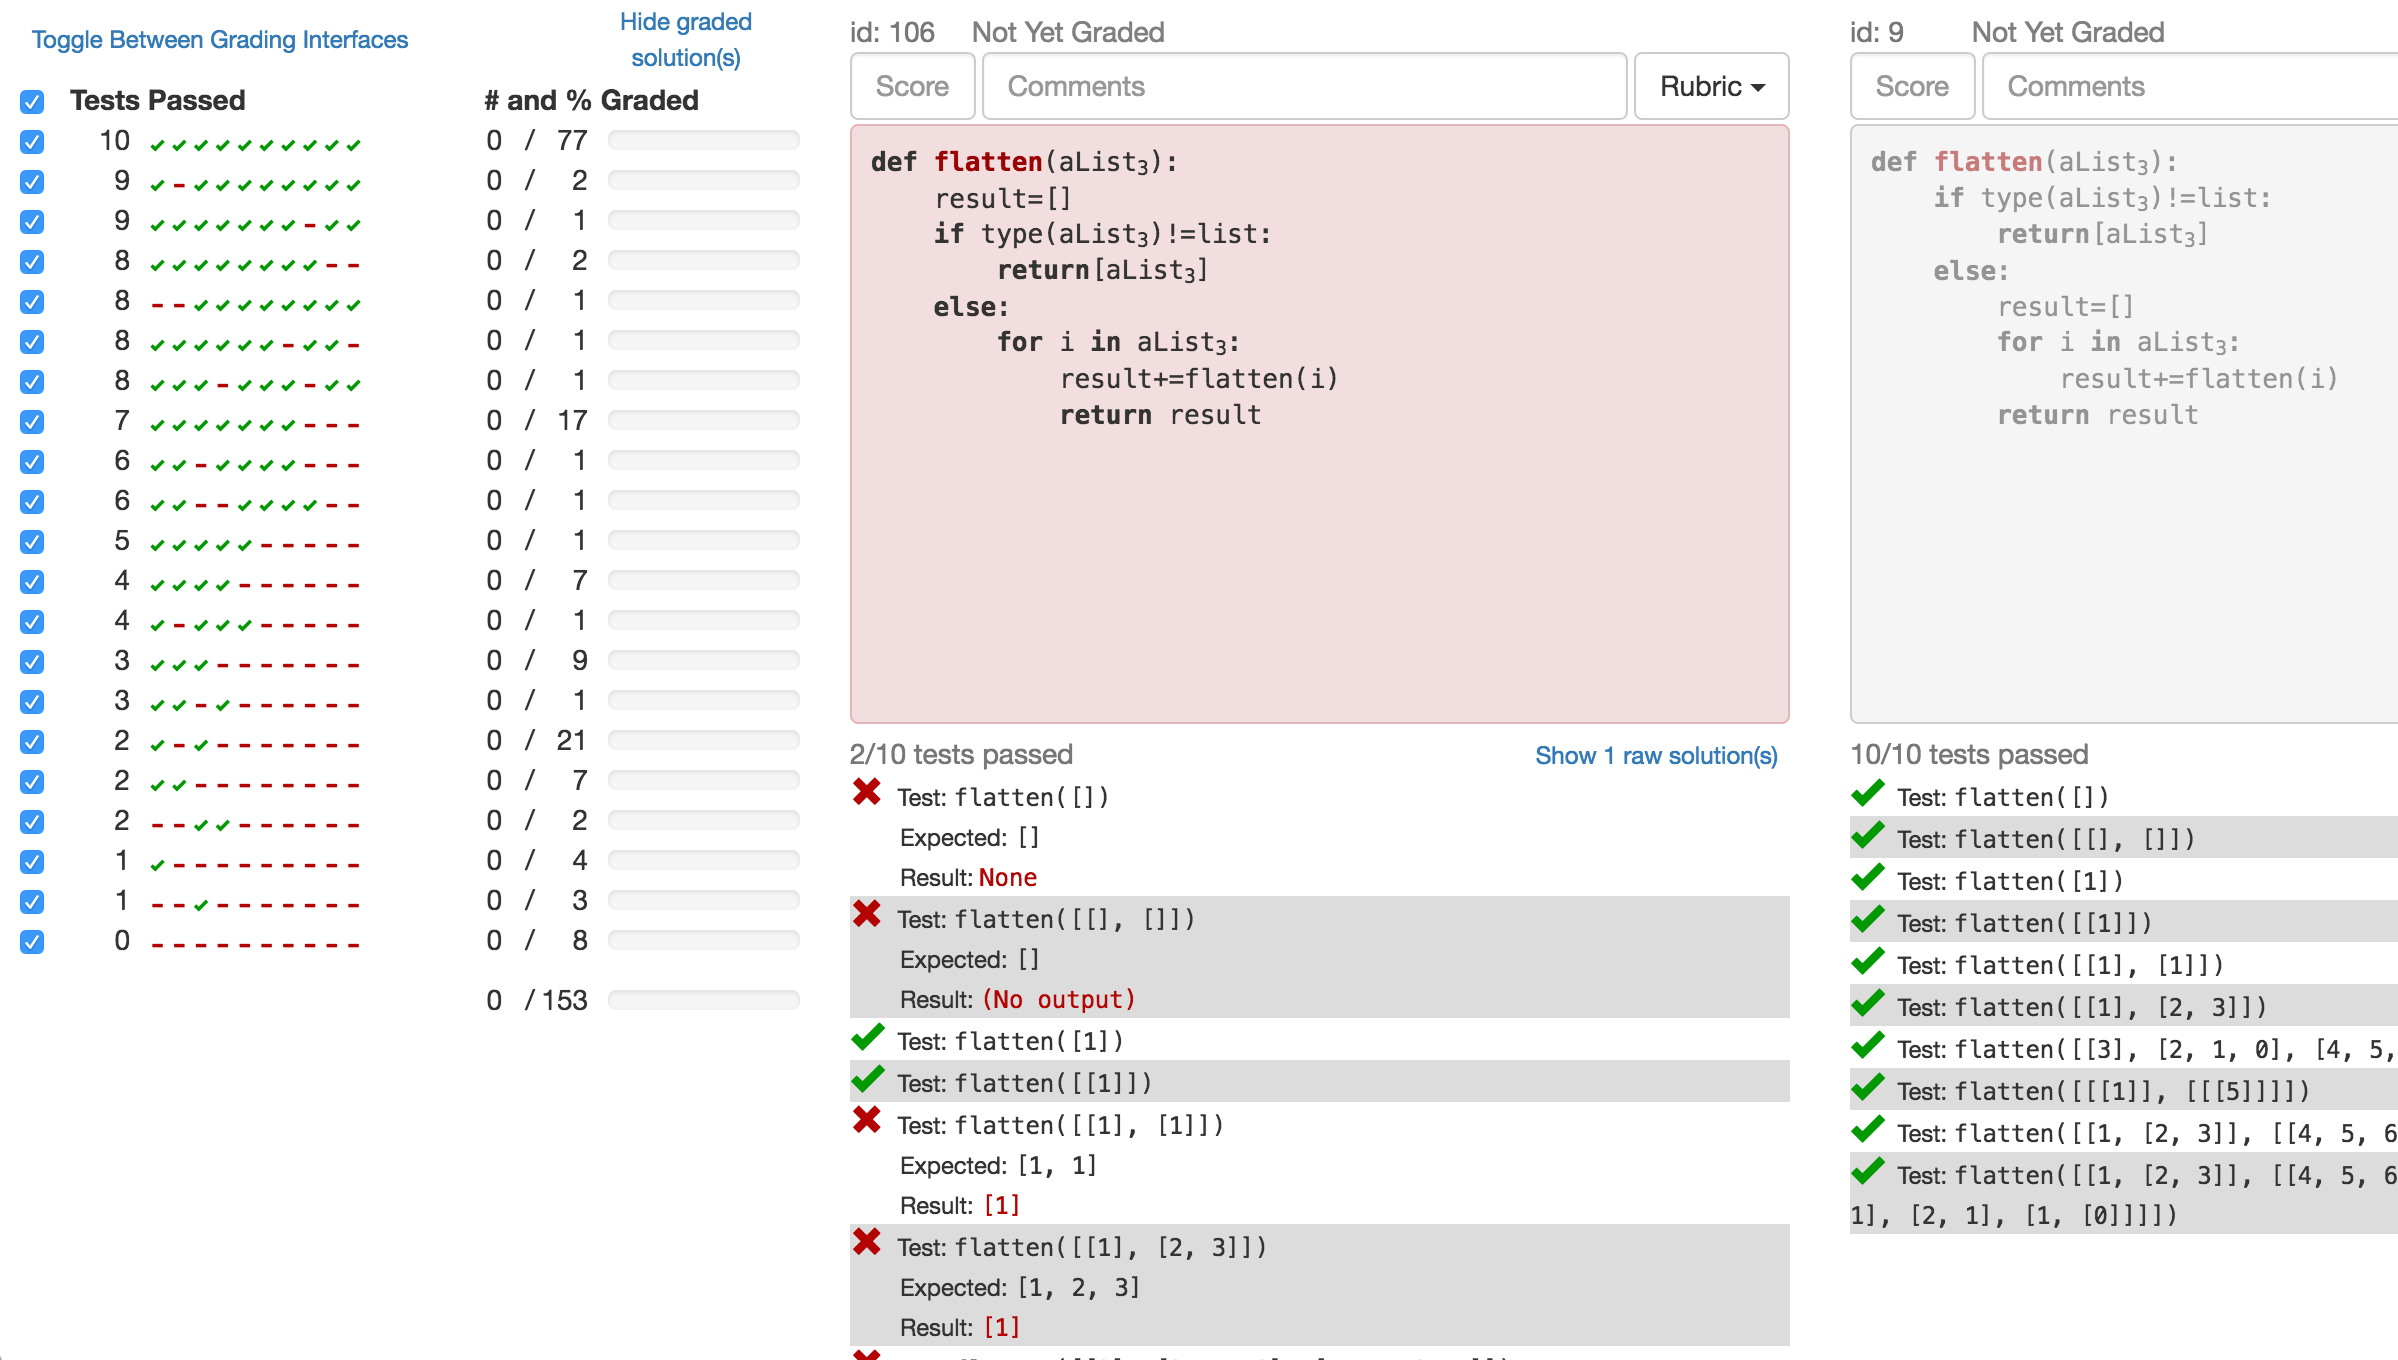
\includegraphics[width=\textwidth]{Body/figures/grovercode/figure_1}
\caption{The GroverCode user interface displaying solutions to an introductory Python programming exam problem, in which students are asked to implement a function to flatten a nested list of arbitrary depth.
}
\label{fig:whole_interface}
\end{figure} \todo{cite Stacey's thesis and Been's thesis for any borrowed figures}

\begin{figure}
\centering
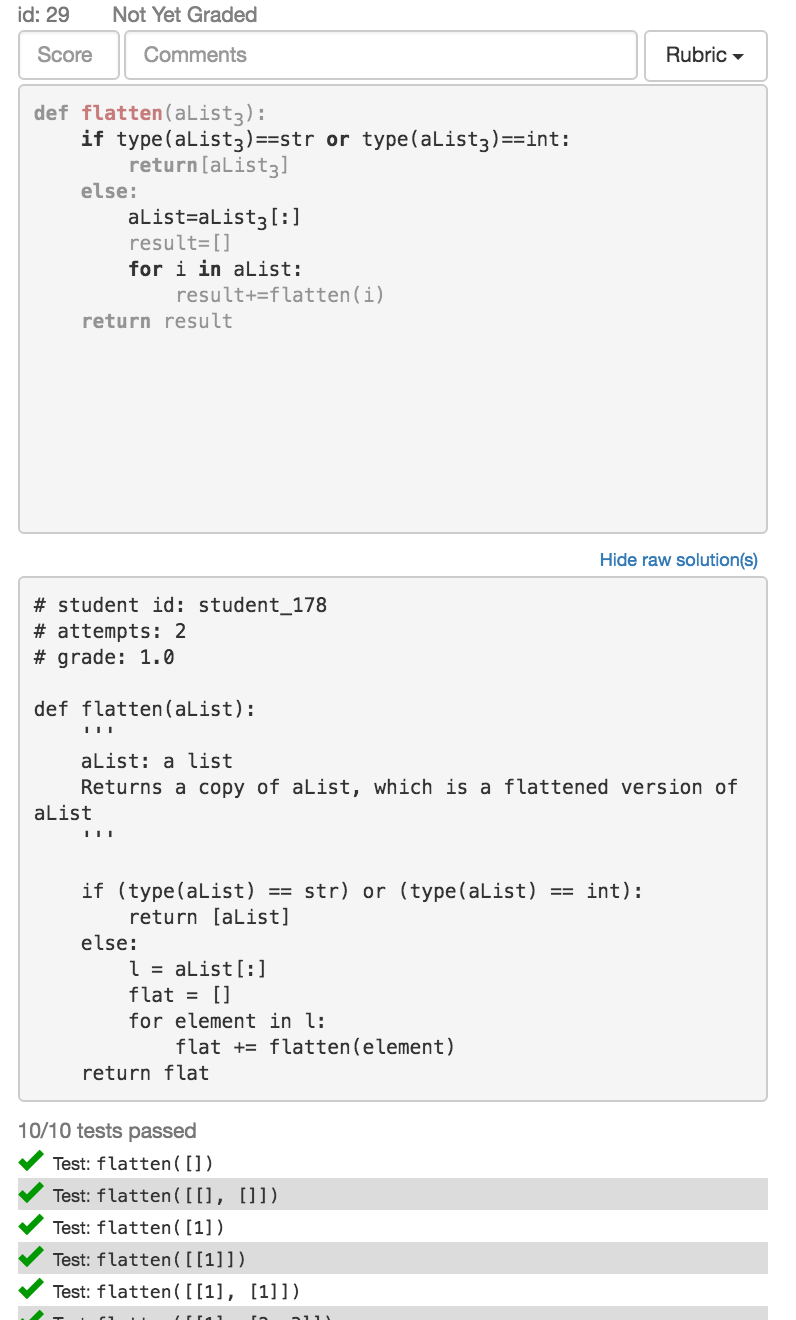
\includegraphics[width=0.5\textwidth]{Body/figures/grovercode/figure_2}
\caption{A correct solution, its corresponding raw submission, and its performance on test cases, as displayed in GroverCode.}
\label{fig:correct_stack}
\end{figure}
 
\begin{figure}
\centering
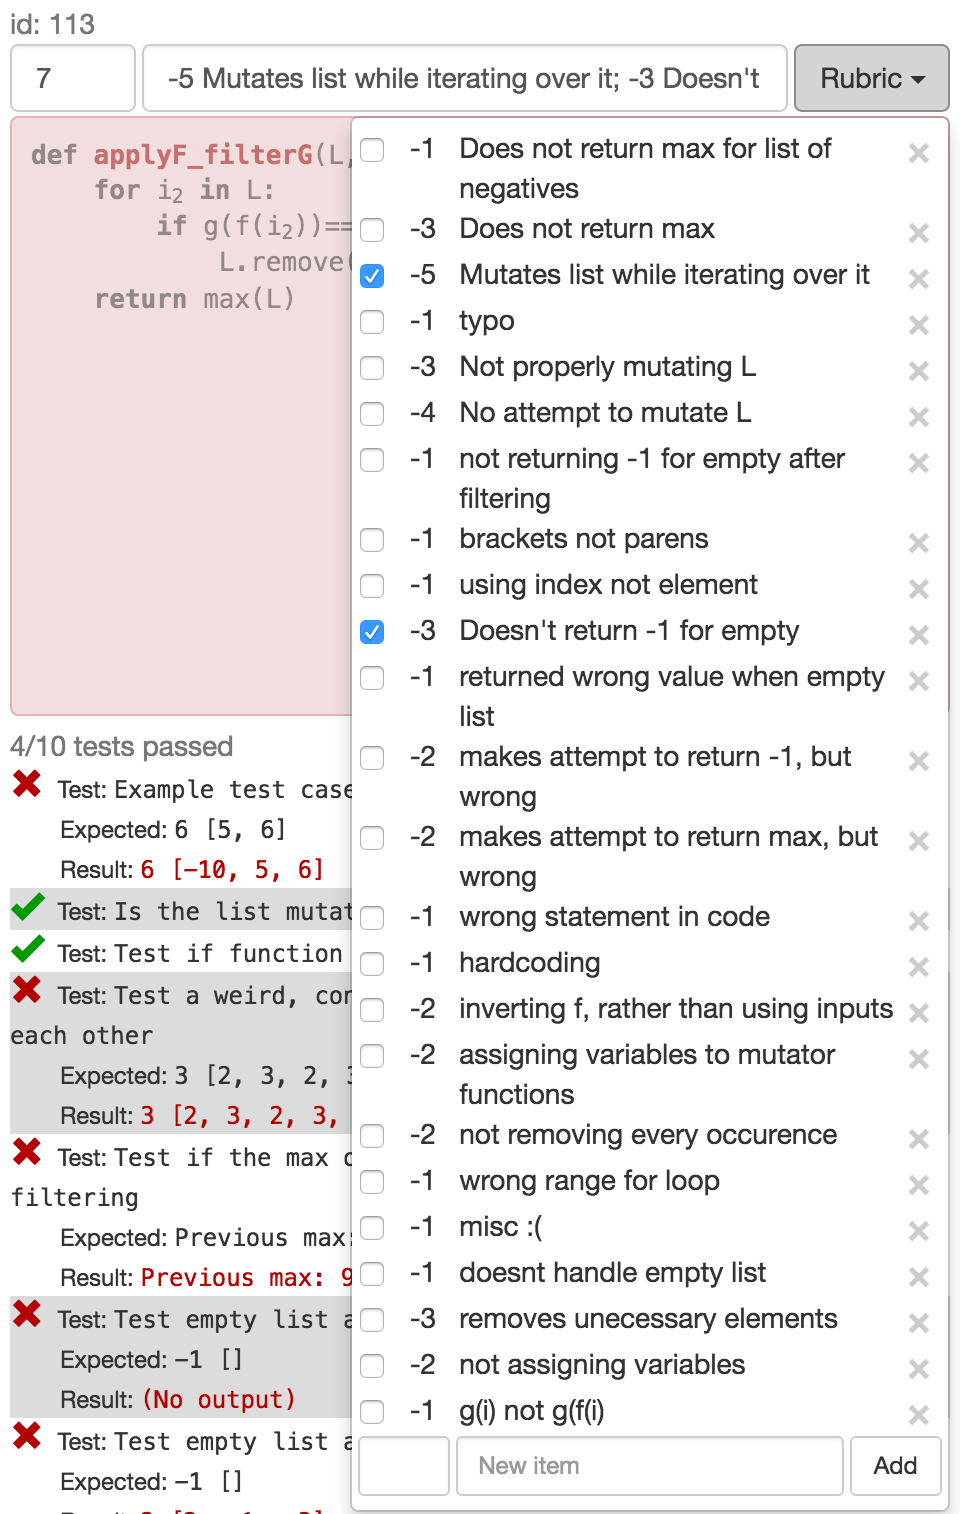
\includegraphics[width=0.5\textwidth]{Body/figures/grovercode/figure_3}
\caption{A stack with the rubric dropdown menu open. Text for each of the checked items is automatically inserted in the comment box.}
\label{fig:rubric}
\end{figure}


\subsection{Implementation}~\label{subsec:grovercodepipeline}

The GroverCode implementation is a modification of the OverCode pipeline, including the updates described in Section~\ref{subsec:morelineinfo}. Solutions which return an expected output for all test cases during the preprocessing step are categorized as "correct", and all other solutions, having failed at least one test case, are categorized as "incorrect". Correct solutions are canonicalized by the same process as was used in the original OverCode. 

In the original OverCode pipeline for correct solutions, variable behavior is assumed to hold enough semantic information to be the sole basis on which variable names are canonicalized. In this first version of GroverCode, applies this rule to incorrect solutions as well, but only for variables whose behavior matches a common variable in the correct solutions. %if a variable in an incorrect solution has the same behavior as a common variable in the correct solutions, GroverCode will rename the variable in the incorrect solution so it matches the common variable's name in the correct solutions.

However, that purely behavior-based renaming strategy may change in future versions of GroverCode because, given that incorrect solutions are known to be wrong with respect to input-output behavior, the behavior of the variables within them is suspect too, regardless of whether it happens to match a common variable in a correct solution.

Consider the following example: in the syntax of an incorrect solution, a variable $i$ may be operated or depended on exactly the same way as a common variable in a correct solution. However, if an error somewhere else in the solution causes $i$ to behave differently, the original method of variable renaming will be thrown off. Based on this example, variables in incorrect solutions that are not already renamed based on behavior are renamed based on syntax.

The most recently updated OverCode pipeline represents each line's syntax and variables in a separable way (see Section~\ref{subsec:morelineinfo}). The line's syntax, e.g., \texttt{for \underline{\hspace{1em}} in \underline{\hspace{1em}}:}, is referred to as a template. For each common variable in correct solutions, GroverCode counts how many times it appears in each template and in which location, represented as an index into the blanks in the template. Examples of templates and locations are shown in Table~\ref{table:template-location}. 

\begin{table}
\centering
\caption*{\textbf{Example:} All templates and locations in which the abstract variable \texttt{exp}, the second argument to a recursive \texttt{power} function, appears. A location represents the index or indices of the blanks that the abstract variable occupies, where the first blank is index 0, the second is index 1, and so on. The second and third columns together form a template-location pair. Copied with permission from Terman~\cite{staceythesis}}\todo{get explicit permission}
\begin{tabular}{|c|c|c|}
\hline
Example line of code & Template & Location \\
\hline
\texttt{def power(base, exp):} & \texttt{def power(\underline{\hspace{1em}},\underline{\hspace{1em}}):} & 1 \\
\hline
\texttt{while index <= exp:} & \texttt{while \underline{\hspace{1em}}<=\underline{\hspace{1em}}:} & 1 \\
\hline
\texttt{return 1.0*base*power(base, exp-1)} & \texttt{return 1.0*\underline{\hspace{1em}}*\underline{\hspace{1em}}*power(\underline{\hspace{1em}},\underline{\hspace{1em}}-1)} & 3 \\
\hline
\texttt{return base*power(base, exp-1)} & \texttt{return \underline{\hspace{1em}}*power(\underline{\hspace{1em}},\underline{\hspace{1em}}-1)} & 2 \\
\hline
\texttt{return power(base, exp-1)*base} & \texttt{return power(\underline{\hspace{1em}},\underline{\hspace{1em}}-1)*\underline{\hspace{1em}}} & 1 \\
\hline
\texttt{ans = base*power(base, exp-1)} & \texttt{\underline{\hspace{1em}}=\underline{\hspace{1em}}*power(\underline{\hspace{1em}},\underline{\hspace{1em}}-1)} & 3 \\
\hline
\texttt{if exp <= 0:} & \texttt{if \underline{\hspace{1em}}<=0:} & 0 \\
\hline
\texttt{if exp == 0:} & \texttt{if \underline{\hspace{1em}}==0:} & 0 \\
\hline
\texttt{if exp >= 1:} & \texttt{if \underline{\hspace{1em}} >= 1:} & 0 \\
\hline
\texttt{assert type(exp) is int and exp >= 0} & \texttt{assert type(\underline{\hspace{1em}}) is int and \underline{\hspace{1em}}>=0} & 0, 1 \\
\hline
\end{tabular}
\label{table:template-location}
\end{table}

If a yet-unrenamed variable in an incorrect solution appears in the exact same template-locations as a common variable in a correct solution, it will be renamed to match that common variable.

If a variable in an incorrect solution is still not canoncialized, the counts of template-locations associated with each common variable in the correct solutions are used, as described in detail in Terman~\cite{staceythesis}, to infer the most likely common variable it could be renamed to, as long as a threshold for similarity is met. Otherwise, its original name is kept. 

\subsection{Field Deployment}

The GroverCode analysis pipeline was run on both the midterm and final exam problems from the Spring 2016 semester of 6.0001, which had approximately 200 students enrolled. These exams contained seven programming problems in total, and between 133 and 189 solutions per problem made it through the analysis pipeline to be displayed in the user interface. 

Using the GroverCode user interface, nine instructors, including one lecturer and eight teaching assistants (TAs) graded these solutions as part of their official grading responsibilities. Those solutions that did not successfully pass through the pipeline were graded by hand afterwards.

The TAs' grading events, e.g., adding or applying rubric items and point values to solutions, were logged. An observer took extensive notes during each day-long grading session to capture spontaneous feature requests as well as bugs and complaints. For full disclosure, one of the TAs in these grading sessions was the Masters of Engineering student who implemented most of GroverCode, and the observer was the author of this thesis.

%\begin{comment}
\subsubsection{Programming Exam Problems}

For each problem processed during the field deployments, an example of a staff-written correct solution is included below. Given the increasing difficulty of these exam problems, the following numbers dropped between the midterm and the final: the number of students present to take the exam, the number of students who submitted any solution to a given problem before the test period ended, and the number of correct solutions that could be clustered.

{\bf Midterm Problems}

\begin{itemize}
\item Question 4: \texttt{power}. Write a recursive function to calculate the exponential \texttt{base} to the power \texttt{exp}.

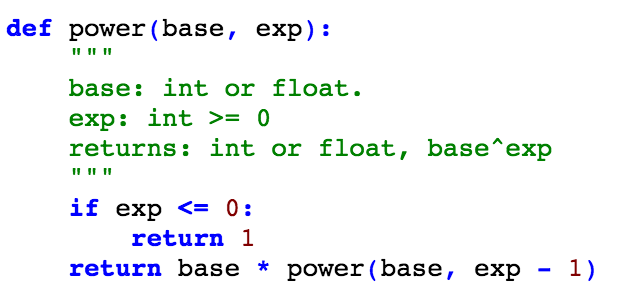
\includegraphics[scale=0.65]{Body/figures/grovercode/fig_power}

\item Question 5: \texttt{give\_and\_take}. Given a dictionary \texttt{d} and a list \texttt{L}, return a new dictionary that contains the keys of \texttt{d}. Map each key to its value in \texttt{d} plus one if the key is contained in \texttt{L}, and its value in d minus one if the key is not contained in \texttt{L}.

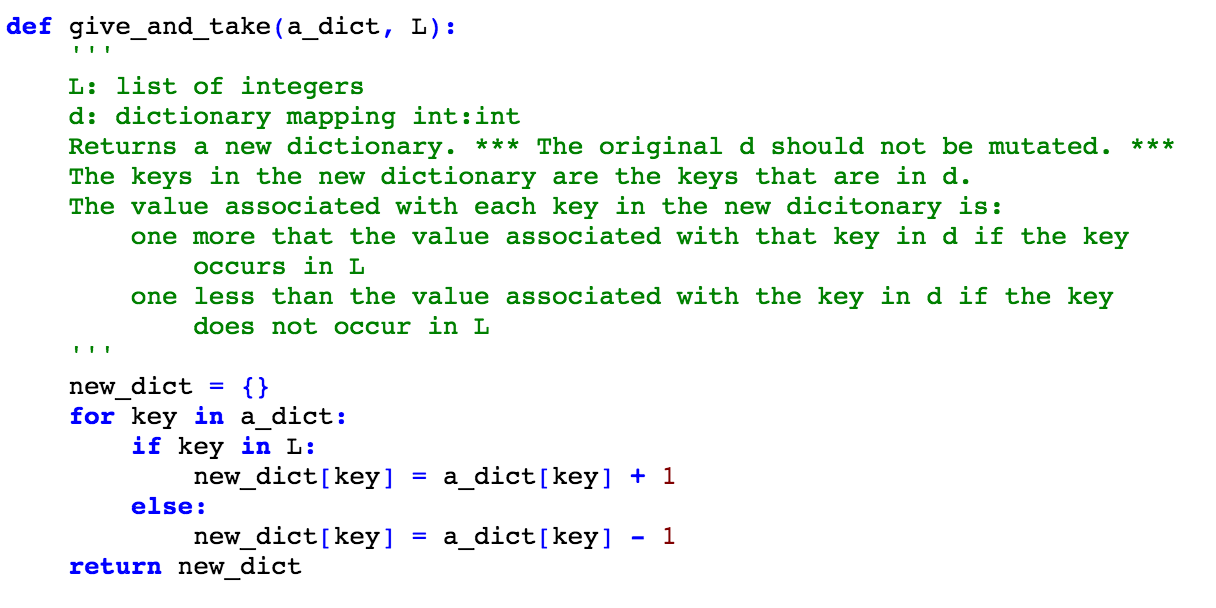
\includegraphics[scale=0.65]{Body/figures/grovercode/fig_give_and_take}

\item Question 6: \texttt{closest\_power}. Given an integer base and a target integer \texttt{num}, find the integer exponent that minimizes the difference between \texttt{num} and \texttt{base} to the power of exponent, choosing the smaller exponent in the case of a tie.

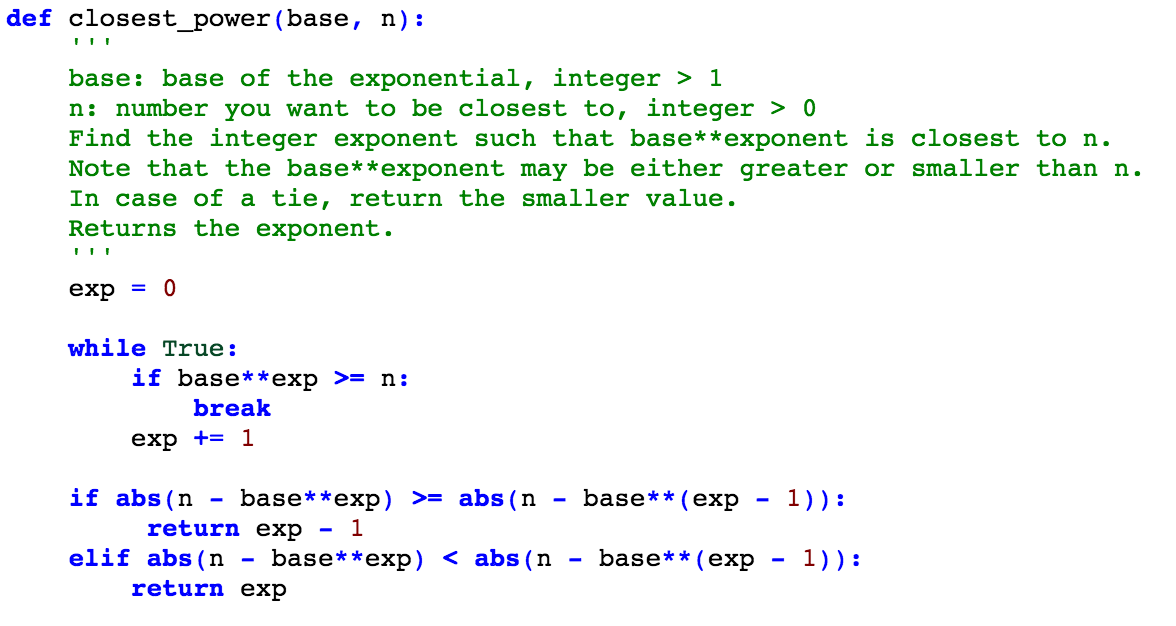
\includegraphics[scale=0.65]{Body/figures/grovercode/fig_closest_power}
\end{itemize}

{\bf Final Exam Problems}

\begin{itemize}
\item Question 4: \texttt{deep\_reverse}. Write a function that takes a list of lists of integers \texttt{L}, and reverses \texttt{L} and each element of \texttt{L} in place.

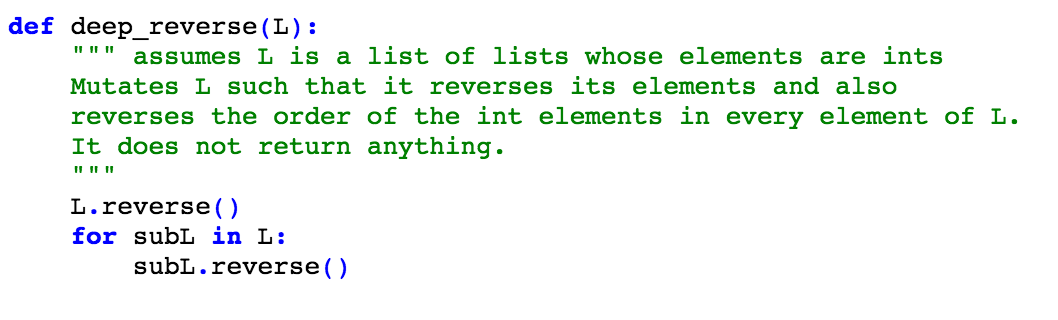
\includegraphics[scale=0.65]{Body/figures/grovercode/fig_deep_reverse}

\item Question 5: \texttt{applyF\_filterG}. Write a function that takes three arguments: a list of integers \texttt{L}, a function \texttt{f} that takes an integer and returns an integer, and a function \texttt{g} that takes an integer and returns a boolean. Remove elements from \texttt{L} such that for each remaining element \texttt{i}, \texttt{f(g(i))} returns \texttt{True}. Return the largest element of the mutated list, or -1 if the list is empty after mutation.

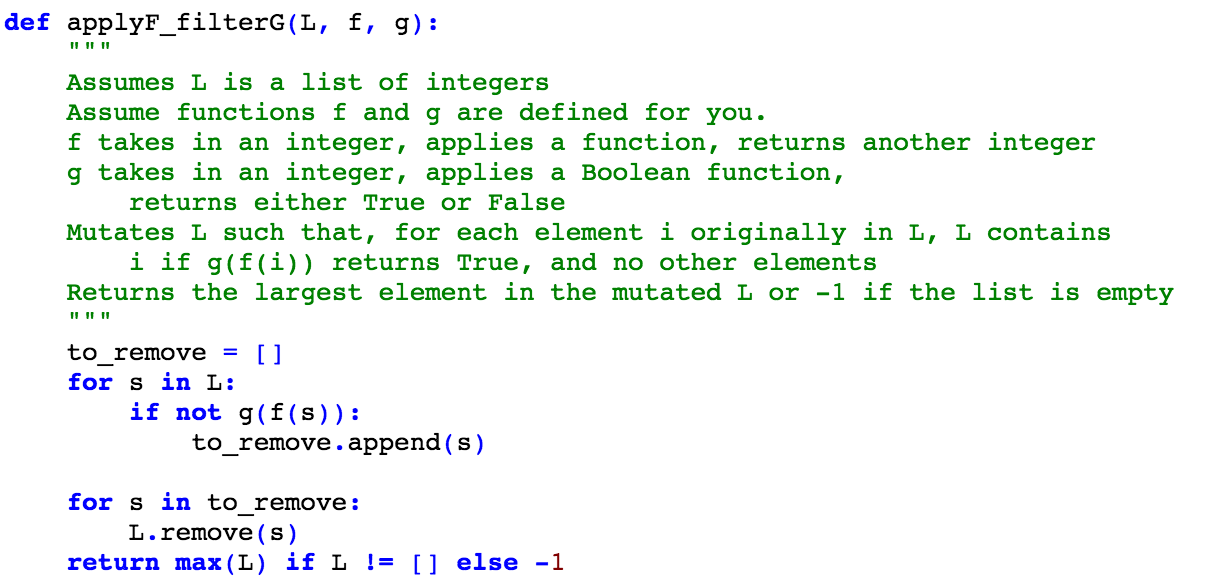
\includegraphics[scale=0.65]{Body/figures/grovercode/fig_applyF_filterG}

\item Question 6: \texttt{MITCampus}. Given the definitions of two classes: \texttt{Location}, which represents a two-dimensional coordinate point, and \texttt{Campus}, which represents a college campus centered at a particular \texttt{Location}, fill in several methods in the \texttt{MITCampus} class, a subclass of \texttt{Campus} that represents a college campus with tents at various \texttt{Locations}.

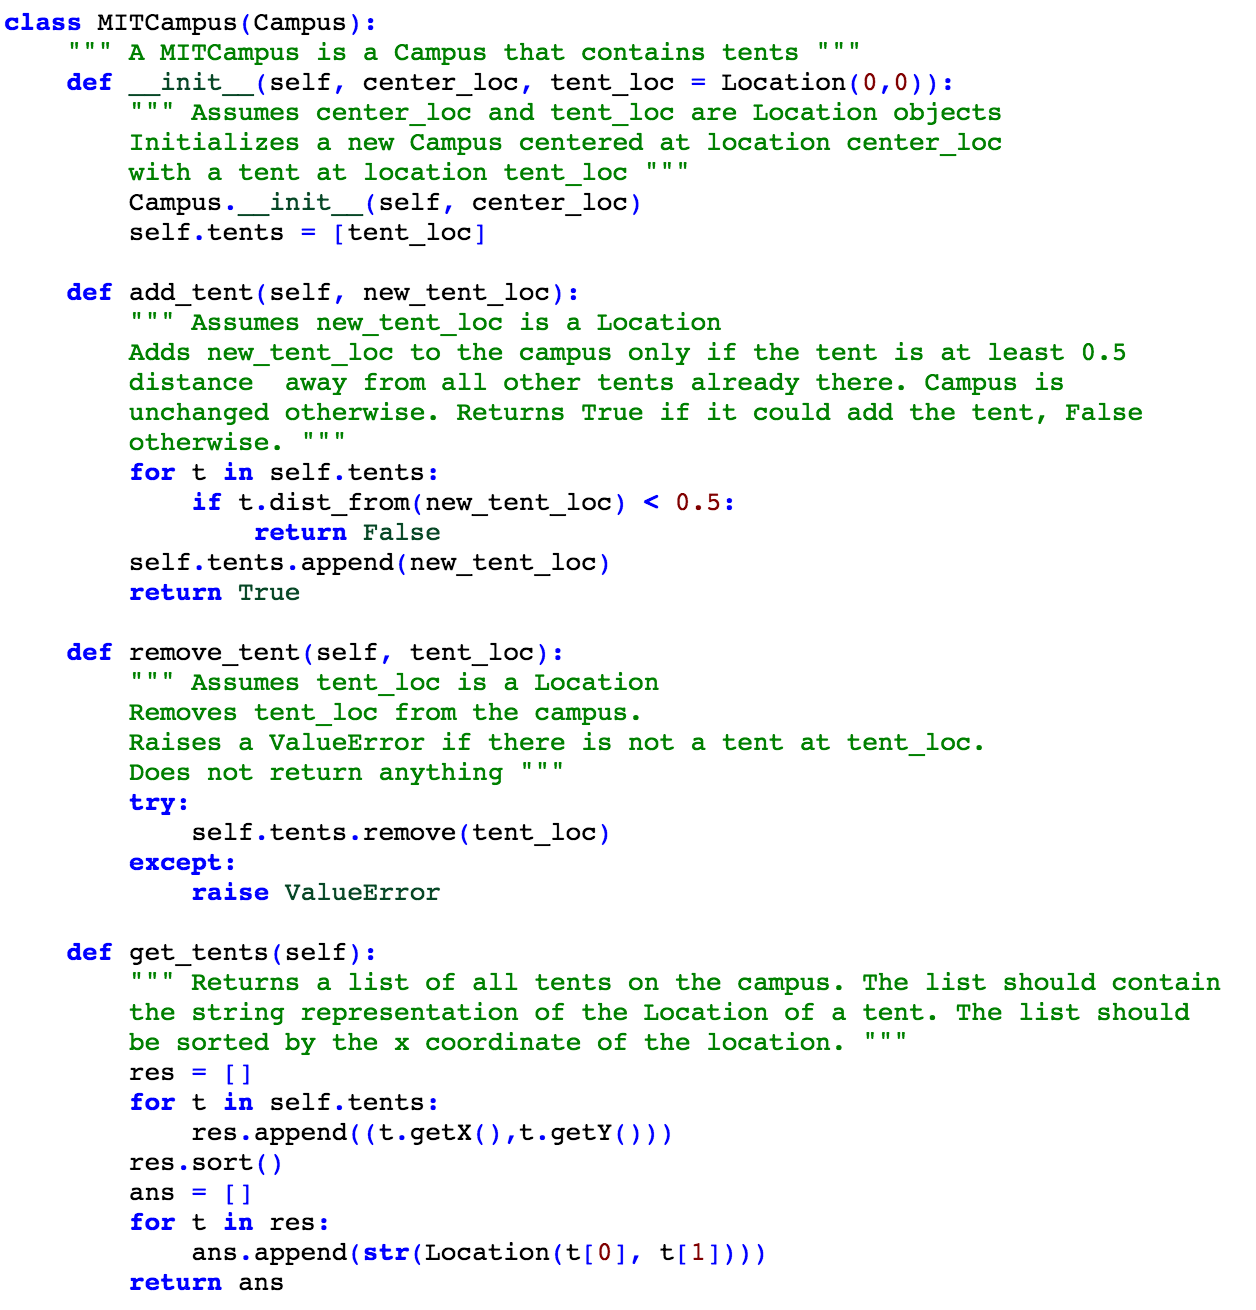
\includegraphics[scale=0.65]{Body/figures/grovercode/fig_mitcampus}

\item Question 7: \texttt{longest\_run}. Write a function that takes a list of integers \texttt{L}, finds the longest run of either monotonically increasing or monotonically decreasing integers in \texttt{L}, and returns the sum of this run.

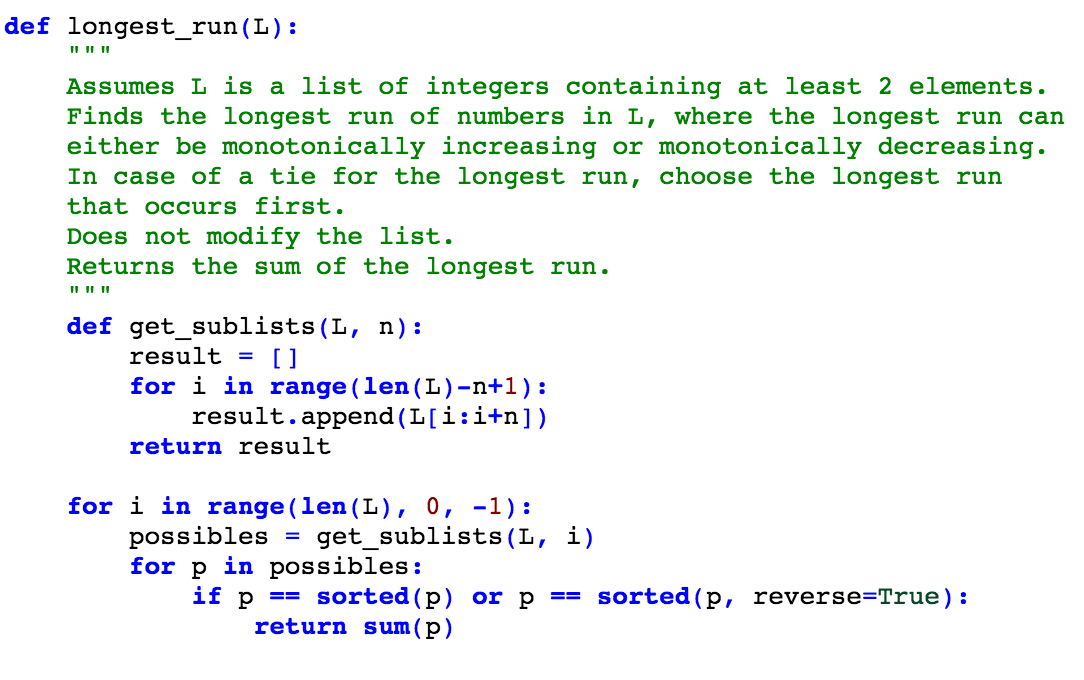
\includegraphics[scale=0.65]{Body/figures/grovercode/fig_longest_run}
\end{itemize}

\subsubsection{Pipeline Evaluation}

The number of submissions submitted for each problem and the number that were successfully processed by the GroverCode pipeline is shown in Table~\ref{table:num_submissions}.

\begin{table}[h!]
\centering
\begin{tabular}{|c|c|c|c|c|c|c|c|}
\hline
& \multicolumn{3}{c|}{Quiz} & \multicolumn{4}{c|}{Final} \\
\cline{2-8}
& q4 & q5 & q6 & q4 & q5 & q6 & q7 \\
\hline
Submissions & 193 & 193 & 193 & 175 & 173 & 170 & 165 \\
\hline
Mean lines per submission & 9.9 & 16.9 & 19.8 & 12.3 & 20.9 & 50.0 & 41.8 \\
\hline
Solutions successfully processed & 186 & 189 & 168  & 170 & 166  & 134 & 133 \\
 & (96\%) & (98\%) & (87\%) & (97\%) & (96\%) & (79\%) & (81\%) \\
\hline
\end{tabular}
\caption{Number of submissions submitted and successfully processed  by GroverCode for each problem in the dataset. Reasons why a solution might not make it through the pipeline include syntax errors and memory management issues caused by students' inappropriate function calls.}
\label{table:num_submissions}
\end{table}



Table~\ref{table:cluster_stats} captures the scale of the variation as well as some clustering statistics.

\begin{table}[!ht]
\centering
\begin{tabular}{|l|c|c|c|c|c|c|c|}
\hline
& \multicolumn{3}{c|}{Quiz} & \multicolumn{4}{c|}{Final} \\
\cline{2-8}
& q4 & q5 & q6 & q4 & q5 & q6 & q7 \\
\hline
Correct submissions & 182 & 160 & 94 & 96 & 49 & 16 & 12 \\
 & (94\%) & (82\%) & (49\%) & (55\%) & (28\%) & (9\%) & (7\%) \\
\hline
Incorrect submissions & 4 & 29 & 74 & 74 & 117 & 118 & 121 \\
\hline
Test cases & 10 & 15 & 25 & 11 & 10 & 17 & 28 \\
\hline
Distinct error signatures & 6 & 16 & 36 & 12 & 38 & 57 & 42 \\
\hline
Correct stacks & 40 & 84 & 93 & 47 & 46 & 16 & 12 \\
\hline
Stacks containing > 1 submission & 13 & 18 & 1 & 8 & 2 & 0 & 0 \\
\hline
Solutions collapsed into stacks & 151 & 94 & 2 & 57 & 5 & 0 & 0 \\
\hline
\end{tabular}
\caption{The degree of variation in input-output behavior and statistics about stack sizes.}
\label{table:cluster_stats}
\end{table}


%\begin{comment}
Table~\ref{table:renametype} summarizes the counts of the various mechanims by which variables in incorrect solutions were canonicalized.

\begin{table}
\centering
\begin{tabular}{|l|c|c|c|c|c|c|c|}
\hline
& \multicolumn{3}{c|}{Quiz} & \multicolumn{4}{c|}{Final} \\
\cline{2-8}
& q4 & q5 & q6 & q4 & q5 & q6 & q7 \\
\hline
Vars. in incorrect submissions & 15 & 149 & 482 & 289 & 550 & 559 & 859 \\
\hline
Vars. renamed based on values & 14 & 84 & 266 & 97 & 246 & 97 & 187 \\
\hline
Vars. renamed based on templates & 0 & 58 & 166 & 136 & 264 & 188 & 489 \\
\hline
Vars. not renamed & 1 & 7 & 50 & 56 & 40 & 274 & 183 \\
\hline
\end{tabular}
\caption{Statistics about variables renaming based on different heuristics in the GroverCode canonicalization process.}
\label{table:renametype}
\end{table}
%\end{comment}
 
\subsubsection{Discussion}
For simpler solutions, variable renaming was an invisible and possibly slightly confusing helping hand. One grader remarked, outloud: "Why is everyone naming their iterator variable 'i'?" at which point he had to be reminded of the variable renaming process. As solutions became more varied and structurally complex, graders started immediately looking the raw solutions because the renaming of variables, removal of comments, and standardization of whitespace in the canonicalized solutions was removing clues they needed in order to understand the student's intent.

While it was difficult to get direct feedback on the helpfulness of pair-wise difference highlighting and optimized solution ordering, graders heavily used and appreciated the ability to filter and grade solutions one error vector at a time. At least one grader remarked aloud that it seemed like many of the solution with the same error vector made similar mistakes. Therefore filtering by error vector may have been one of the stronger contributors to any hypothetical decreased cognitive load due to using GroverCode over the status quo of random assignment to solutions in a CSV file.

\todo{add to related work Appropriately chosen latent variable models have already been used in the past to model open-source code and answers to open-response mathematical questions.}

\section{Conclusion}
The clustering described in the original OverCode work was relatively limited in scope, but it did produce, at least for simple introductory Python programming problems, a concise standardized representation of solutions that can be used for more statistically sophisticated clustering techniques and as a starting point for helping graders understand and grade incorrect student solutions by hand.

